%%%%%%%%%%%%%%%%%%%%%%%%%%%%%%%%%%%%%%%%%%%%%%%%%%%%%%%
%% Engineer & Master Thesis, LaTeX Template          %%
%% Copyleft by Piotr Woźniak & Artur M. Brodzki      %%
%% Faculty of Electronics and Information Technology %%
%% Warsaw University of Technology, Warsaw, 2019     %%
%%%%%%%%%%%%%%%%%%%%%%%%%%%%%%%%%%%%%%%%%%%%%%%%%%%%%%%

\documentclass[
    left=2.5cm,         % Sadly, generic margin parameter
    right=2.5cm,        % doesnt't work, as it is
    top=2.5cm,          % superseded by more specific
    bottom=3cm,         % left...bottom parameters.
    bindingoffset=6mm,  % Optional binding offset.
    nohyphenation=true % You may turn off hyphenation, if don't like. =false
]{eiti/eiti-thesis} % bazuje na clasie mwart


%\usepackage[
%    backend=bibtex,
%    style=ieee
%]{biblatex}
\usepackage{csquotes}

\langpol % Dla języka angielskiego mamy \langeng
\graphicspath{{img/}}             % Katalog z obrazkami.
%\addbibresource{bibliografia.bib} % Plik .bib z bibliografią

% dodanie kropki po numerze w~LoL https://tex.stackexchange.com/questions/597350/add-dot-after-number-of-listing-in-list-of-listings
\makeatletter
\xpatchcmd\lst@MakeCaption{\protect\numberline{\thelstlisting}\lst@@caption}{\protect\numberline{\thelstlisting.}\lst@@caption}{}{}
%\makeatother
%\makeatletter
%\xpatchcmd{\LT@c@ption}{\protect\numberline{\thetable}}{\protect\numberline.{. \thetable . }}{}{}
\makeatother

\begin{document}

%--------------------------------------
% Strona tytułowa
%--------------------------------------
%\MasterThesis % dla pracy inżynierskiej mamy, tutaj praca koncowa
\EngineerThesis
\instytut{Telekomunikacji}

\title{
    Projekt i wdrożenie systemu bezpieczeństwa \\ 
    sieciowego w środowisku lokalnym z \\
    wykorzystaniem konteneryzacji \\
    wersja 05.2025
}

\engtitle{ % Tytuł po angielsku do angielskiego streszczenia
    Design and Implementation of a Network Security \\
    System in a Local Environment \\ 
    Using Containerization
}

\author{Łukasz Dejko (1203175)}

\promotor{dr inz. Jędrzej Bieniasz}

\date{\the\year}
\maketitle

%--------------------------------------
% Streszczenie po polsku
%--------------------------------------
\streszczenie Celem niniejszej pracy jest zaprojektowanie, wdrożenie oraz omówienie funkcjonalności kompleksowego systemu bezpieczeństwa sieciowego w środowisku lokalnym. System ten integruje mechanizmy ochrony warstwy DNS, filtrowanie ruchu HTTP, monitorowanie aktywności sieciowej, detekcję zagrożeń w czasie rzeczywistym oraz centralne gromadzenie i wizualizację danych telemetrycznych. Kluczowym założeniem projektu było wykorzystanie otwartoźródłowego oprogramowania oraz konteneryzacja usług przy użyciu platformy Docker, co zapewnia modularność, izolację oraz możliwość łatwego zarządzania środowiskiem.

Zastosowane komponenty umożliwiają kontrolę nad dostępem do sieci, blokowanie podejrzanych domen, analizę pakietów w czasie rzeczywistym oraz monitorowanie stanu systemu i usług. W pracy szczegółowo opisano konfigurację elementów odpowiedzialnych za filtrowanie DNS, wykrywanie intruzów, analizę logów oraz ich prezentację w formie czytelnych wykresów i pulpitów zarządczych. System został uruchomiony na serwerze domowym z systemem Linux oraz dodatkowo na platformie Raspberry Pi, co pokazuje elastyczność rozwiązania.

Projekt udowadnia, że także w warunkach domowych możliwe jest wdrożenie systemu bezpieczeństwa opartego na najlepszych praktykach znanych z infrastruktury korporacyjnej. Przedstawione podejście może stanowić punkt wyjścia do dalszych rozważań na temat bezpieczeństwa rozproszonych środowisk cyfrowych oraz implementacji polityk bezpieczeństwa opartych na danych telemetrycznych i analizie zagrożeń.

\slowakluczowe bezpieczeństwo sieci, DNS, Docker, analiza logów, filtracja treści, detekcja zagrożeń, Raspberry Pi, monitoring systemu

\newpage

%--------------------------------------
% Streszczenie po angielsku
%--------------------------------------
\abstract The purpose of this thesis is to design, implement, and analyze a comprehensive local network security system that integrates DNS-layer protection, HTTP traffic filtering, real-time network activity monitoring, threat detection, and centralized telemetry data visualization. A key objective of the project was the exclusive use of open-source software and containerization via the Docker platform, enabling modularity, service isolation, and ease of management across a distributed architecture.

The implemented solution allows full control over network access, blocking of suspicious domains, real-time traffic analysis, and detailed monitoring of system and service health. The thesis outlines the configuration of components responsible for DNS filtering, intrusion detection, log collection, and interactive dashboards. The system runs on a Linux-based home server and Raspberry Pi, demonstrating its adaptability and cost efficiency.

This work demonstrates that enterprise-grade security practices can be effectively replicated in a domestic setting using widely available technologies. The proposed solution can serve as a starting point for exploring secure digital environments and implementing policy-driven security based on telemetry data and behavioral threat analytics.
\keywords network security, DNS, Docker, log analysis, content filtering, threat detection, Raspberry Pi, system monitoring
\newpage

%--------------------------------------
% Oświadczenie o autorstwie
%--------------------------------------
%\makeauthorship
%\blankpage

%--------------------------------------
% Spis treści
%--------------------------------------
\thispagestyle{empty}
\tableofcontents
%\blankpage

%--------------------------------------
% Rozdziały
%--------------------------------------
\newpage 
\section{Praefatio}
\lipsum[1-2] Aaaa \cite{goossens93}.

\begin{figure}[!h]
	\label{fig:486dx2}
	\centering 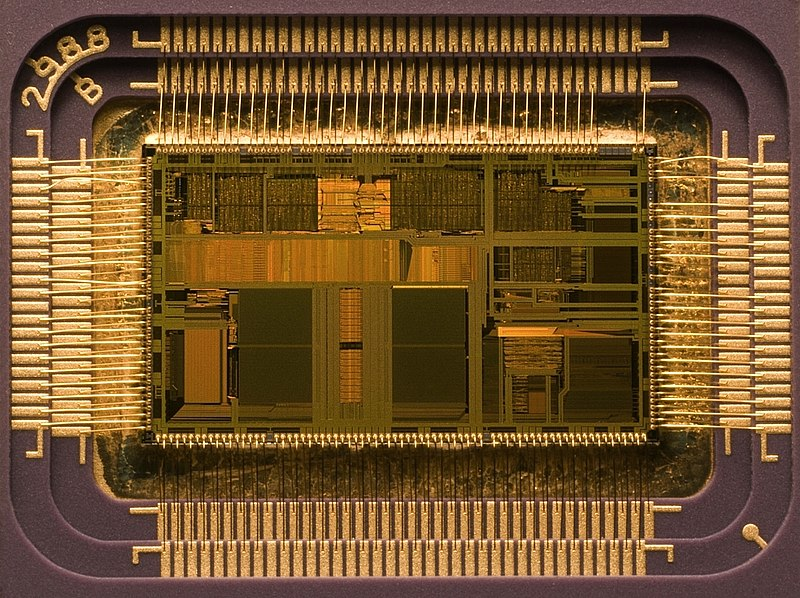
\includegraphics[width=0.5\linewidth]{80486dx2.jpg}
	\caption{Procesor Intel 80486DX2 \cite{Wiki:486dx2}}
\end{figure}

\lipsum[3-4]

%%%%%%%%%%%%%%%%%%%%%%%%%%%%%%%%%%%%%%%%%%%%%%%%%%%%%%%%%%%%%%%%%

\section{De Finibus Bonorum et Malorum}
\lipsum[1] Lorem ipsum .}. 
\begin{align*}
	E & = mc^2 \\ 
	y & = ax^2 + bx + c
\end{align*}

\lipsum[3]

\begin{align}
	\begin{bmatrix}
		1 & 0 & 0 \\ 
		0 & 2 & 0 \\ 
		0 & 0 & 3
	\end{bmatrix} \cdot 
	\begin{bmatrix}
		4 \\ 5 \\ 6
	\end{bmatrix} = 
	\begin{bmatrix}
		4 \\ 10 \\ 18
	\end{bmatrix}
\end{align}

\lipsum[4] Lorem ipsum dolor sit amet, consectetur adipiscing elit, sed do eiusmod tempor incididunt ut labore et dolore magna aliqua \cite{szczypiorski2015}, \cite{duqu2011}, \cite{shs2015}, \cite{wozniak2018}, \cite{dcp19}. 

\subsection{Critique of Pure Reason}
\kant[1]

\begin{table}[!h] \label{tab:tabela1} \centering
	\caption{Przykładowa tabela}
	\begin{tabular} {| c | c | r |} \hline
		Kolumna 1 & Kolumna 2 & Liczba \\ \hline\hline
		cell1 & cell2 & 60 \\ \hline
		cell4 & cell5 & 43 \\ \hline
		cell7 & cell8 & 20,45 \\ \hline
		\multicolumn{2}{|r|}{Suma:} & 123,45 \\ \hline
	\end{tabular}
\end{table}

\kant[2]

\begin{longtable}{| c | m{0.58\linewidth} | r | m{0.1\linewidth} |} 
	\caption{Tabela wielostronicowa} \\ 
	\hline
	Lp & \multicolumn{1}{c|}{Treść} & \multicolumn{1}{c|}{Kwota} & \multicolumn{1}{m{0.1\linewidth}|}{Wariant opłaty} \\ \hline\hline \endfirsthead
	
	\endfoot
	\hline \endlastfoot
	
	1 & Lorem ipsum dolor sit amet, consectetur adipiscing elit, sed do eiusmod tempor incididunt ut labore et dolore magna aliqua. & 111 111,11 zł & \multicolumn{1}{c|}{WAR1} \\ \hline
	2 & Lorem ipsum dolor sit amet, consectetur adipiscing elit, sed do eiusmod tempor incididunt ut labore et dolore magna aliqua. & 22 222,22 zł & \multicolumn{1}{c|}{WAR1} \\ \hline
	3 & Lorem ipsum dolor sit amet, consectetur adipiscing elit, sed do eiusmod tempor incididunt ut labore et dolore magna aliqua. & 33 333,33 zł & \multicolumn{1}{c|}{WAR1} \\ \hline
	4 & Lorem ipsum dolor sit amet, consectetur adipiscing elit, sed do eiusmod tempor incididunt ut labore et dolore magna aliqua. & 444 444,44 zł & \multicolumn{1}{c|}{WAR1} \\ \hline
	5 & Lorem ipsum dolor sit amet, consectetur adipiscing elit, sed do eiusmod tempor incididunt ut labore et dolore magna aliqua. & 55 555,55 zł & \multicolumn{1}{c|}{WAR1} \\ \hline
	6 & Lorem ipsum dolor sit amet, consectetur adipiscing elit, sed do eiusmod tempor incididunt ut labore et dolore magna aliqua. & 66 666,66 zł & \multicolumn{1}{c|}{WAR1} \\ \hline
	7 & Lorem ipsum dolor sit amet, consectetur adipiscing elit, sed do eiusmod tempor incididunt ut labore et dolore magna aliqua. & 777 777,77 zł & \multicolumn{1}{c|}{WAR1} \\ \hline
	8 & Lorem ipsum dolor sit amet, consectetur adipiscing elit, sed do eiusmod tempor incididunt ut labore et dolore magna aliqua. & 8 888,88 zł & \multicolumn{1}{c|}{WAR1} \\ \hline
	9 & Lorem ipsum dolor sit amet, consectetur adipiscing elit, sed do eiusmod tempor incididunt ut labore et dolore magna aliqua. & 999 999,99 zł & \multicolumn{1}{c|}{WAR1} \\ \hline
	10 & Lorem ipsum dolor sit amet, consectetur adipiscing elit, sed do eiusmod tempor incididunt ut labore et dolore magna aliqua. & 111 111,11 zł & \multicolumn{1}{c|}{WAR2} \\ \hline
	11 & Lorem ipsum dolor sit amet, consectetur adipiscing elit, sed do eiusmod tempor incididunt ut labore et dolore magna aliqua. & 22 222,22 zł & \multicolumn{1}{c|}{WAR2} \\ \hline
	12 & Lorem ipsum dolor sit amet, consectetur adipiscing elit, sed do eiusmod tempor incididunt ut labore et dolore magna aliqua. & 33 333,33 zł & \multicolumn{1}{c|}{WAR2} \\ \hline
	13 & Lorem ipsum dolor sit amet, consectetur adipiscing elit, sed do eiusmod tempor incididunt ut labore et dolore magna aliqua. & 444 444,44 zł & \multicolumn{1}{c|}{WAR2} \\ \hline
	14 & Lorem ipsum dolor sit amet, consectetur adipiscing elit, sed do eiusmod tempor incididunt ut labore et dolore magna aliqua. & 55 555,55 zł & \multicolumn{1}{c|}{WAR2} \\ \hline
	15 & Lorem ipsum dolor sit amet, consectetur adipiscing elit, sed do eiusmod tempor incididunt ut labore et dolore magna aliqua. & 66 666,66 zł & \multicolumn{1}{c|}{WAR2} \\ \hline
	& \multicolumn{1}{r|}{\textbf{Suma:}} & \textbf{7 777 777,77 zł} & 
	\label{table:koszty}
\end{longtable}
\kant[4]

\subsection{Categorical Imperative}
As any dedicated reader can clearly see, the Ideal of practical reason is a representation of, as far as I know, the things in themselves; as I have shown elsewhere, the phenomena should only be used as a canon for our understanding:
% Parametr label ustawia symbol, a leftmargin - wielkość wcięcia.
% Domyślny układ to [---] bez wcięcia, bo tak pan Marcin Woliński powiedział;
% ale ja nie polecam. // AB
\begin{itemize}
	\item Item 1:
	\begin{itemize}[label=---]
		\item item 1.1;
		\item item 1.2;
		\item item 1.3;
	\end{itemize}
	\item Item 2;
	\item Item 3;
	\item Item 4.
\end{itemize}

\kant[2]
\begin{enumerate}
	\item Item 1:
	\begin{enumerate}
		\item item 1.1;
		\item item 1.2:
		\begin{enumerate}
			\item item 1.2.1;
			\item item 1.2.2;
		\end{enumerate}
		\item item 1.3;
	\end{enumerate}
	\item Item 2;
	\item Item 3;
	\item Item 4.
\end{enumerate}

\kant[9]

\subsection{G\"odel's ontological proof}
\kant[9] Lorem ipsum dolor sit amet, consectetur adipiscing elit, sed do eiusmod tempor incididunt ut labore et dolore magna aliqua \cite{benzmuller2014}, \cite{goedel95}, \cite{wang97}, \cite{koons2005}. 
\begin{assumption} \label{ass:1}
	$ [\![ \ \phi \ ]\!] \Longrightarrow [\![ \ P(\phi); \neg P(\phi) \ ]\!]$
\end{assumption}
\begin{axiom}[Dualność] \label{axiom:1}
	$\neg P(\phi) \Leftrightarrow P(\neg \phi)$, równoważnie $P(\phi) \Leftrightarrow \neg P(\neg \phi)$
\end{axiom}
\begin{axiom}[Całkowitość] \label{axiom:2}
	$ \left( P(\phi) \wedge \forall x: \phi(x) \Rightarrow \psi(x) \right) \Rightarrow P(\psi) $
\end{axiom}
\begin{axiom}[Absolutność] \label{axiom:3}
	$ P(\phi) \Rightarrow \Box P(\phi) $
\end{axiom}
\begin{definition} \label{def:1}
	$ G(x) \Leftrightarrow \forall \phi: \left( P(\phi) \Rightarrow \phi(x) \right) $
\end{definition}
\begin{definition} \label{def:2}
	$ \phi \ ess \ x \Leftrightarrow \phi(x) \wedge \forall \psi \left( \psi(x) \Rightarrow \Box \forall y \left( \phi(y) \Rightarrow \psi(y) \right) \right)  $
\end{definition}
\begin{axiom} \label{axiom:4}
	P(G)
\end{axiom}
\begin{lemma} \label{lemma:1}
	$ P(\phi) \Rightarrow \Diamond \exists x : \phi(x) $
\end{lemma}
\begin{proof}
	Dowód pomijamy, bo jest trywialny :)
\end{proof}
\begin{lemma} \label{lemma:2}
	$ \Diamond \exists x : G(x) $
\end{lemma}
\begin{proof}
	Natychmiastowy wniosek z aksjomatu \ref{axiom:4} i lematu \ref{lemma:1}.
\end{proof}
\begin{lemma} \label{lemma:3}
	$ G(x) \Rightarrow G \ ess \ x $
\end{lemma}
\begin{proof}
	Poprzez podstawienie do definicji \ref{def:2}. 
\end{proof}
\begin{definition} \label{def:3}
	$ E(x) \Leftrightarrow \forall \phi \left( \phi \ ess \ x \Rightarrow \Box\ \exists x: \phi(x) \right) $
\end{definition}
\begin{axiom} \label{axiom:5}
	P(E)
\end{axiom}
\begin{theorem}
	$ \Box\ \exists x : G(x) $
\end{theorem}
\begin{proof}
	Na podstawie definicji \ref{def:1}, lematu \ref{lemma:3} i aksjomatu \ref{axiom:5}. 
\end{proof}

%%%%%%%%%%%%%%%%%%%%%%%%%%%%%%%%%%%%%%%%%%%%%%%%%%%%%%%%%%%%%%%%%

\section{Code listings}
\lipsum[10]

\begin{lstlisting}[language=HTML]
	<html>
	<head>
		<title>Hello world!</title>
	</head>
	<body>
		Hello
	</body>
	</html>
\end{lstlisting}

\lipsum[11]

\begin{lstlisting}[language=C]
	#include <stdio.h>
	int main() {
		// printf() displays the string inside quotation
		printf("Hello world!");
		return 0;
	}
\end{lstlisting}

\lipsum[12]

%%%%%%%%%%%%%%%%%%%%%%%%%%%%%%%%%%%%%%%%%%%%%%%%%%%%%%%%%%%%%%%%%

\section{Dodatkowe informacje}
Informacje jak pisać pracę dyplomową oraz szablon pracy zostały wzięte ze strony \href{http://www.ii.pw.edu.pl/ii_pol/Instytut-Informatyki/Nauczanie/Poradnik-dyplomanta/Przygotowanie-pracy-dyplomowej}{http://www.ii.pw.edu.pl/}.

Jak wygląda proces dyplomowania w~IT można dowiedzieć się na stronie \href{https://secure.tele.pw.edu.pl/wp-content/uploads/2017/06/PROCES-DYPLOMOWANIA-17L.pdf}{https:// secure.tele.pw.edu.pl/} w~sekcji Dydaktyka > Dla studentów > Proces dyplomowania.

Aby zacytować artykuł z~Wikipedii, w~łatwy sposób można uzupełnić bibliografię o~tę pozycję. Na stronie z~wybranym artykułem np. o~\href{https://pl.wikipedia.org/wiki/LaTeX}{Latex} ależy po lewej stronie  wybrać 
\textit{Narzędzia:Cytowanie tego artykułu} i~otrzymamy gotowy 
\href{https://pl.wikipedia.org/w/index.php?title=Specjalna:Cytuj&page=LaTeX&id=58147357}{Przypis do tej strony} \cite{Wiki:Latex}. Na innych stronach należy szukać \textit{bibtex}, \textit{cite} lub podobne.

\subsection{Rysunki}
\begin{figure}[h]
	\centering
	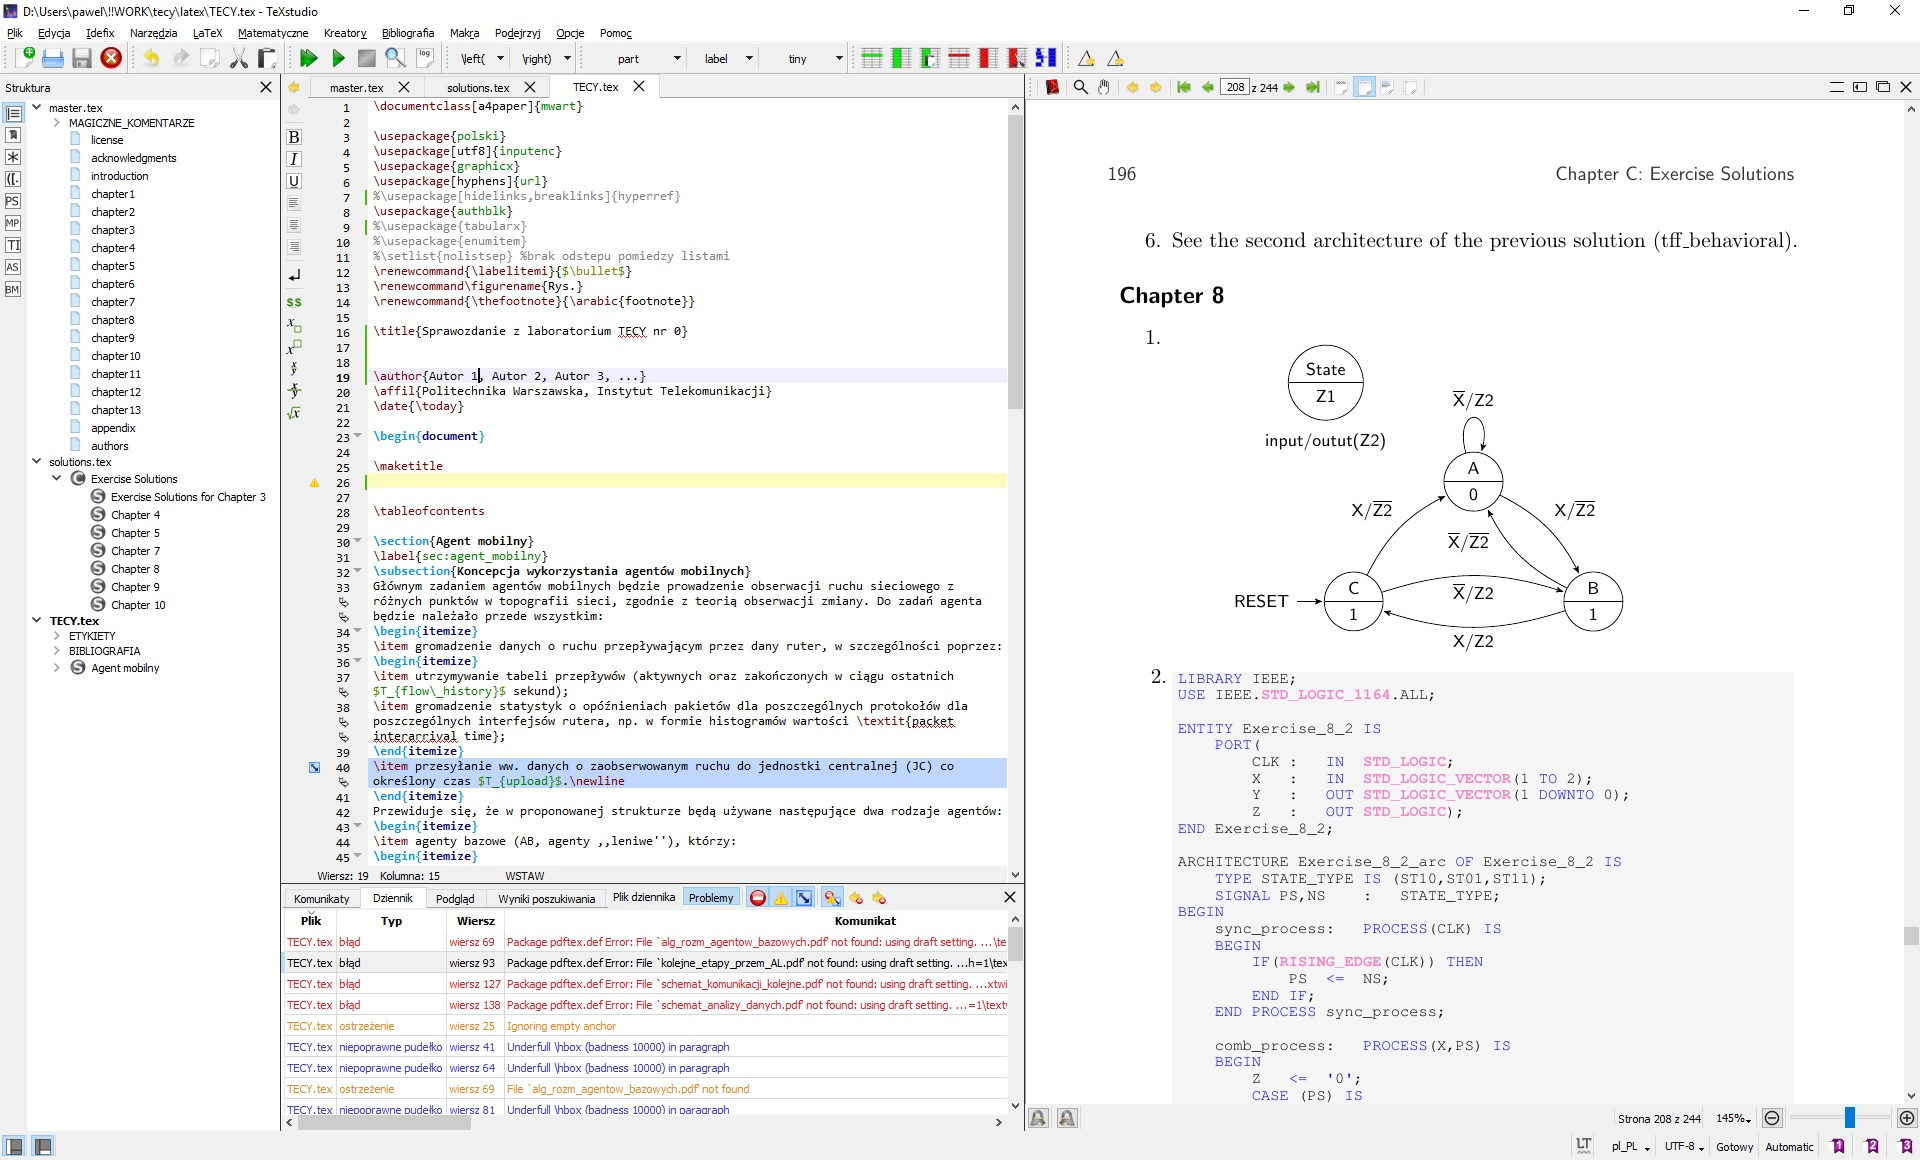
\includegraphics[width=0.5\textwidth]{rysunek_1.jpg}
	\caption{\label{fig:rysunek_1}Widok edytora TeXstudio \cite{TeXstudio}}
\end{figure}
\FloatBarrier %zatrzymanie przenoszenia rysunku

\subsection{Tablice}
\begin{table}[h]
	\begin{center}
		\caption{Przykładowa tabela}
		\label{tab:tabela_przyklad}
		\begin{tabular}{|r|l|c|c|}
			\hline 
			Miejsce & Drużyna & Gole & Punkty \\
			\hline \hline
			1 & Legia & 12 & 36 \\
			2 & Górnik & 10 & 30 \\
			3 & Widzew & 8 & 24\\
			4 & ŁKS & 7 & 21 \\ \hline
		\end{tabular}
	\end{center}
\end{table}
\FloatBarrier %zatrzymanie przenoszenia rysunku

\subsection{Wydruki}
\begin{lstlisting}[label=lst:wydruk,caption={Testowy program w Verilog},language=Verilog,numbers=left]
	module lfsr_4 //rejestr o dlugosci 4
	#(parameter n=4)
	(
	input clk,
	input a_reset,
	input load,
	input [n-1:0]  a,
	output [n-1:0] result
	);
	
	reg [n-1:0] register;
	
	always@(posedge clk, posedge a_reset)
	if(a_reset)
	register <= 0;
	else 
	if(load)
	register <= 1; // inicjacja
	else
	register <= {register[0],register[3:2], register[1]^register[0]};
	
	assign result = register;
	
	endmodule
\end{lstlisting}

\subsection{Matematyka}
Przykład użycia trybu matematycznego (poniżej).

The mass-energy equivalence is described by the famous equation

$$E=mc^2$$ %wysrodkowany bez numeracji

discovered in 1905 by Albert Einstein. 
In natural units ($c$ = 1), the formula expresses the identity %w tekscie

\begin{equation} %wysrodkowany z numeracja
	E=m
\end{equation}

\subsection{Oprogramowanie - wersja Windows}
\label{sec:oprogramowanie}
Do pracy w środowisku \LaTeXe{} (wersja aktualnie używana) proponuję (wybór subiektywny i~jedynie słuszny) następujący zestaw oprogramowania \cite{Ghostscript, MikTeX, TeXstudio}, instalacja w takiej kolejności:
\begin{itemize}
	\item Ghostscript -- interpreter plików PostScript i PDF  \url{https://www.ghostscript.com/},
	\item MikTeX -- dystrybucja dla Windows  \url{https://miktex.org/} - zestaw narzędzi,
	\item Adobe Reader -- przeglądarka plików PDF \url{https://acrobat.adobe.com/pl/pl/},
	\item TeXstudio -- edytor i kompilator \url{https://texstudio.org/},
	\item (opcjonalnie) Słownik PL do edytora -- należy zaimportować w edytorze (rys. \ref{fig:rysunek_spr})  \url{https://extensions.openoffice.org/en/project/polish-dictionary-pack},
	\item (opcjonalnie) Java JRE (do uruchomienia LT) \url{https://www.java.com/pl/download/},
	\item (opcjonalnie) Narzędzie Language Tool -- można uruchomić \textit{off-line} w edytorze \url{https://languagetool.org/download/LanguageTool-4.6.zip},
\end{itemize}

\begin{figure}[h]
	\centering
	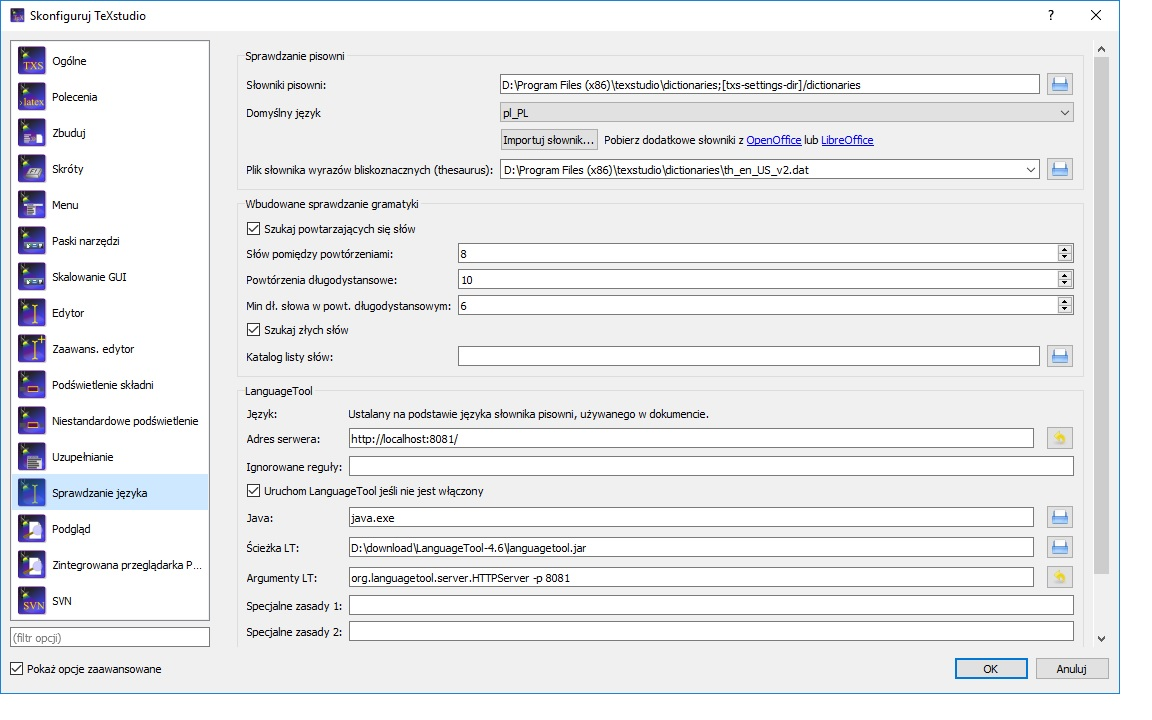
\includegraphics[width=1\textwidth]{texstudio_sprawdzanie_jezyka.jpg}
	\caption{\label{fig:rysunek_spr}Widok edytora TeXstudio -- ustawianie opcji do sprawdzania języka}
\end{figure}

Jeżeli kompilacja pierwszego dokumentu nie przebiegnie prawidłowo, tzn. kompilator nie znajdzie czcionek, należy uruchomić program \texttt{updmap.exe} z~pakietu MikTex.

Dla zawansowanych: sposób na automatyczne dodawanie tabulatora po literach a, i, o, u,w, z aby nie zostawały na końcu linii -- sierotki. Wyzwalacz \textit{trigger} ma postać \begin{verbatim}
	(?language:latex)\sa\s|\si\s|\so\s|\su\s|\sw\s|\sz\s
\end{verbatim}

\begin{figure}[h]
	\centering
	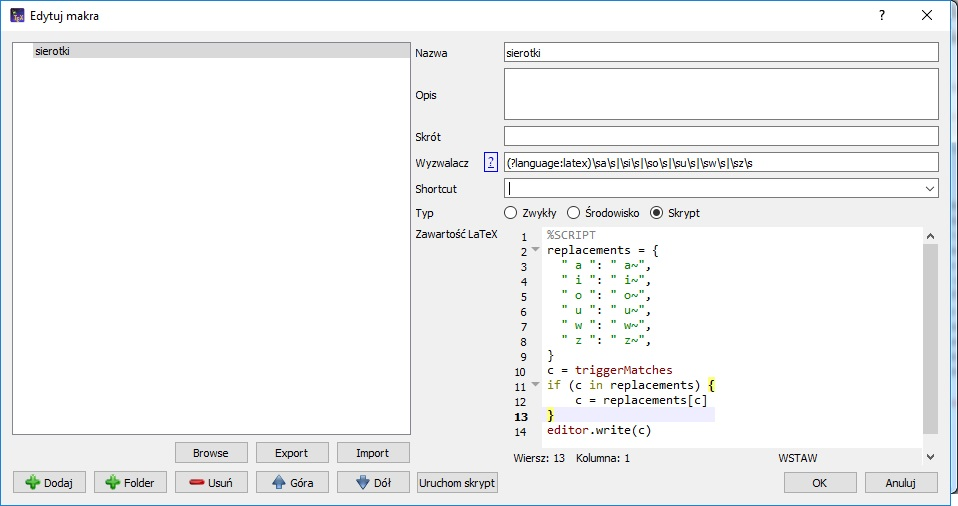
\includegraphics[width=1\textwidth]{sierotki.jpg}
	\caption{\label{fig:sierotki}Widok edytora TeXstudio -- makro dla sierotek}
\end{figure}

\begin{lstlisting}[label=lst:sierotki,caption={Widok edytora TeXstudio -- dodanie makra do sierotek},numbers=left]
	%SCRIPT
	replacements = {
		" a ": " a~",
		" i ": " i~",
		" o ": " o~",
		" u ": " u~",
		" w ": " w~",
		" z ": " z~",
	}
	c = triggerMatches
	if (c in replacements) {
		c = replacements[c]
	}
	editor.write(c)
\end{lstlisting}


\subsection{Inne strony}
\begin{itemize}
	\item Obowiązkowa lektura: \url{ftp://ftp.gust.org.pl/TeX/info/lshort/polish/lshort2e.pdf}	
	\item \url{http://www.mif.pg.gda.pl/homepages/sylas/students/wdi/index.html},
	\item \url{https://www.mimuw.edu.pl/~mbodnar/prosem/wprowadzenie_v2016.pdf}	
	\item \url{http://latex-kurs.x25.pl//}
	\item \url{https://matematyka.pl/viewtopic.php?t=28951}	
	\item \url{https://pl.wikibooks.org/wiki/LaTeX}	
	\item \url{https://en.wikibooks.org/wiki/LaTeX}
	\item Edytor i kompilator \textit{on-line} Overleaf -- także do pracy grupowej \url{https://www.overleaf.com/}
	\item \url{https://www.google.com/search?q=latex+tutorial+pl} \dots	
\end{itemize}

%%%%%%%%%%%%%%%%%%%%%%%%%%%%%%%%%%%%%%%%%%%%%%%
\section{Summatio}      % Ale można też pisać w jednym. 
\kant[5-6]

%--------------------------------------------
% Literatura
%--------------------------------------------
\newpage
%\printbibliography
\bibliographystyle{plabbrv} % plplain plabbrv plalpha
\bibliography{bibliografia.bib}
% Załączniki

\newpage
\section*{Nazwa załącznika 1}
\lipsum[1]

\newpage
\section*{Nazwa załącznika 2}
\lipsum[1]

\newpage

\end{document} % Dobranoc. 

